\newpage

\subsection{Praktikos metu naudotos technologijos}
Šiame poskyryje aprašomos technologijos, kurias naudojau praktikos metu ir pavyzdžiai, kur jos buvo naudojamos. 
Atlikdamas praktiką mobiliųjų įrenginių kūrimo komandoje, turėjau galimybę dirbti su įvairiomis pripažintomis ir naujausiomis mobiliųjų programėlių kūrimo technologijomis. Toliau aprašoma pagrindinių \enquote{Android} ir \enquote{iOS} technologijų, kuriomis naudojausi, apžvalga:

\subsubsection{Kotlin}
Kotlin yra viena iš populiariausių programavimo kalbų kuriant Android mobiliąsias programėles. Lyginant su Java programavimo kalba, Kotlin yra modernesnė, null reikšmių saugumu. Kotlin lengvai pritaikoma senesniuose projektuose, parašytuose su Java ir XML vartotojo sąsaja, paprasta atnaujinti seną kodo bazę. Sintaksės panašumas į kitas programavimo kalbas, padeda lengvai ir greita išmokti Kotlin programavimo kalbos pagrindus.
Visos praktikos metu Kotlin programavimo kalbą naudojau kurti naudotojo sąsajos logiką, tvarkyti duomenis ir integruoti naujus komponentus į turimą mobiliąją programėlę.

Darbe ši programavimo kalba naudojama Android mobiliosios programėlės kūrime. Su Java programavimo kalba, šiame projekte neteko susidurti. Prieš porą metų buvo permigruota iš Java į Kotlin, nauji komponentai rašomi Kotlin programavimo kalba.
Komandos nariai turi didelę patirtį su Kotlin programavimo kalba, todėl iškilus klausimams, jie gali būti išspręsti greitai ir efektyviai paklausus komandos narių.

\subsubsection{Jetpack Compose}

\enquote{Jetpack Compose} yra Android rekomenduojamas modernus įrankių rinkinys, skirtas vartotojo sąsajai kurti. Rinkinys supaprastina ir pagreitina Android mobiliųjų programėlių vartotojo sąsajos kūrimą. Šiame karkase vartotojo sąsaja konstruojama deklaratyviai. Taikant šią paradigmą kodas gali būti glaustesnis ir lengviau suprantamas.

Projekte šis karkasas dar yra tik pradedamas naudoti kuriant naujus komponentus, kurie bus naudojami programėlėje, programuojami su šiuo karkasu. Šiuo metu yra tik 1 itin patyręs programuotojas, kuris kūrė pačius pirmuosius Jetpack Compose komponentus, paruošė testavimo mobiliąją programėlę. Kiti programuotojai skatinami mokytis šio karkaso, paskirti laiko darbo metu mokymuisi. 

% % \begin{figure}
% %     \centering
% %     \begin{minted}[linenos,tabsize=1,breaklines]{kotlin}
% %     @Composable
% %     fun TestListParameterView(
% %         values: List<String>,
% %         initialMessage: String = "Initial message",
% %         labelText: String = "Label",
% %         onRemove: (String) -> Unit,
% %         onAdd: (String) -> Unit
% %     ) {
% %         var text by rememberSaveable { mutableStateOf(initialMessage) }
% %         Column {
% %             LazyColumn(modifier = Modifier.height(200.dp)) {
% %                 items(items = values) { value ->
% %                     Row {
% %                         Text(
% %                             modifier = Modifier.height(44.dp).fillMaxWidth(0.9f),
% %                             maxLines = 2,
% %                             style = MaterialTheme.typography.body2,
% %                             text = value,
% %                             overflow = TextOverflow.Ellipsis
% %                         )
% %                         Spacer(modifier = Modifier.weight(1f))
% %                         TextButton(
% %                             modifier = Modifier.width(44.dp).background(Color.Transparent),
% %                             onClick = { onRemove(value) },
% %                             content = { Icon(painter = painterResource(...)) }
% %                         )
% %                     }
% %                 }
% %             }
% %             OutlinedTextField(
% %                 modifier = Modifier.fillMaxWidth(),
% %                 value = text,
% %                 onValueChange = { text = it },
% %                 label = { Text(labelText) }
% %             )
% %             Button(onClick = {
% %                 if (text.isNotBlank()) {
% %                     onAdd(text)
% %                     text = ""
% %                 }
% %             }) { Text(text = "Add") }
% %         }
% %     }
% %     \end{minted}
% %     \caption{Jetpack Compose programinis kodas}
% %     \label{fig:composeCode}
% % \end{figure}

% % \begin{figure}[htbp!]
% %   \centering
% %   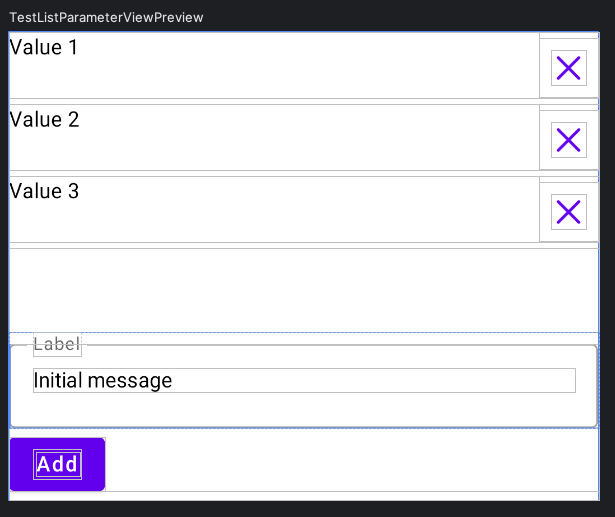
\includegraphics[width=0.8\linewidth]{Images/JetpackCompose.png}
% %   \caption{Jetpack Compose komponento peržiūra}
% %   \label{fig:example}
% % \end{figure}


\subsubsection{Swift}
Swift yra galinga, tačiau nesunki pradedantiesiems programavimo kalba, kurią Apple sukūrė savo įrenginiams. Lyginant su \enquote{Objective-C}, Swift pasižymi švariu ir glaustu stiliumi, artimesniu natūraliai kalbai. Priešingai nei \enquote{Objective-C}, Swift atlieka daugiau automatinio atminties valdymo ir tipų tikrinimo, tai padeda išvengti gedimų ir klaidų, kurios dažniau pasitaiko \enquote{Objective-C} kalboje. Dėl šių priežasčių, programinį kodą  greita parašyti ir lengva prižiūrėti. Nors \enquote{Objective-C} dar naudojama esamuose projektuose, integruoti Swift nesunku net ir į itin senus projektus. Su Swift programavimo kalba galima rašyti programėles iPhone, iPad, MacBook, Apple watch įrenginiams. Neseniai atsiradusiam \enquote{Apple vision pro} prietaisui irgi yra galimybė kurti programas šia programavimo kalba. 

Praktikos metu neteko matyti Objective-C parašyto programinio kodo, vienintelė vieta, kur teko susidurti su šia kalba, tai \enquote{PdfTron} atvirasis programinis kodas. Komandoje programuotojai yra itin patyrę, todėl atsiradus keblumams, galima greitai gauti atsakymus.
\subsubsection{SwiftUI}

\enquote{SwiftUI} - tai naujas Apple karkasas įrenginių naudotojo sąsajų kūrimui. Skirtingai nuo storyboards sąsajų kūrimo, kuris remiasi vizualiniu komponentų dėliojimu ekrane, \enquote{SwiftUI} naudoja deklaratyvų požiūrį. Storyboards vartotojo sąsajos konvertuojamos į XML,  kas yra gana nepatogu, kai atliekamos programinio kodo pakeitimų peržiūros. Kaip ir \enquote{Jetpack Compose}, \enquote{SwiftUI}, kode galima atlikti vartotojo sąsajos būsenų valdymą, deklaratyviai konstruoti vartotojo sąsają. Išbandžius abi technologijas iOS vartotojo sąsajos kūrimo technologijas, norint suprasti ir atlikti kodo pakeitimus esamame projekte, \enquote{SwiftUI} yra geresnis programavimo karkasas, suprasti kodo veikimo principus, prireiks mažiau laiko.

Šis programavimo karkasas projekte pradėtas naudoti tik prieš metus. Tačiau sukurti nauji komponentai, testinė komponentų mobilioji programėlė, parašyti šiuo karkasu. Kadangi \enquote{SwiftUI} yra naujas karkasas, dokumentacija dar nėra tokia išsami, kartais, norint rasti sprendimą, reikia gana intensyviai ieškoti informacijos. Komandoje yra 4 programuotojai, kurie gerai išmano šį karkasą.